
\documentclass[12pt, a4paper]{article}

\usepackage[utf8]{inputenc}
\usepackage[T1]{fontenc}
\usepackage[russian]{babel}
\usepackage[oglav,spisok,boldsect,eqwhole,figwhole,hyperref,hyperprint,remarks,greekit]{./style/fn2kursstyle}
\graphicspath{{./style/}{./figures/}}

\usepackage{multirow}
\usepackage{supertabular}
\usepackage{multicol}
\usepackage{amsmath}
\usepackage{afterpage}
\usepackage{amsmath}
% Параметры титульного листа
\title{Решение уравнения Рейнольдса\\ в рамках теории газовой смазки \\ методом конечных элементов}
\author{В.\,Г.~Пиневич}
\supervisor{А.\,В.~Селиванов}
\group{ФН2-71Б}
\date{2024}

% Переопределение команды \vec, чтобы векторы печатались полужирным курсивом
\renewcommand{\vec}[1]{\text{\mathversion{bold}${#1}$}}%{\bi{#1}}
\newcommand\thh[1]{\text{\mathversion{bold}${#1}$}}
%Переопределение команды нумерации перечней: точки заменяются на скобки
\renewcommand{\labelenumi}{\theenumi)}
\begin{document}

\maketitle

\tableofcontents



\newpage

\section-{Введение}
Задачи расчёта подшипников газодинамического типа с зазорами разнообразной формы до сих пор остаются весьма актуальными. По сути, они сводятся к изучению газового смазочного слоя в тонком зазоре произвольной формы. Решением таких задач занимается гидродинамическая теория смазки. Этот раздел механики жидкости и газа начал развиваться в конце XIX века вслед за потребностями техники. Начало теоретическому исследованию течений в тонких зазорах положили работы Н. П. Петрова и британского учёного Осборна Рейнольдса, уточнённые и доведённые до возможности практического применения А. Зоммерфельдом, А. Мичелем. Дальнейшие исследования позволили распространить результаты созданной Рейнольдсом теории на газодинамические подшипники. Были даже предприняты успешные попытки получения общего вида уравнения Рейнольдса для смазочного слоя без привязки к конкретной системе координат. Данная работа посвящёне получению пригодной к использованию в практических задачах формы уравнения Рейнольдса и решению его методом конечных элементов.


\section{Постановка задачи}
Задача данной работы --- вывести, а затем показать методику решение дифференциального уравнения Рейнольдса методом конечных элементов.
\begin{equation}
	\label{reinolts-task}
\frac{\partial}{\partial x} \left(h^3 \frac{\partial p}{\partial x} \right) + \frac{\partial}{\partial z} \left(h^3 \frac{\partial p}{\partial z} \right) = 6 \mu U \frac{\partial h}{\partial x} \text{, }
\end{equation}
где $h = h(x)$ --- толщина слоя, $p = p(x, z)$ --- давление, $\mu$ --- коэффициент вязкости. Граничные условия: $U$ --- скорость в направлении $x$ на одной из пластин, $p_{\text{в}}$ --- повышенное давление, $p_{\text{н}}$ --- пониженное давление. 

Уравнения будем рассматривать в квадратной области. Схематичное изображение области и граничных условий изображено на рис.~\ref{obl_resh}.

\begin{figure}[!htbp]
	\center{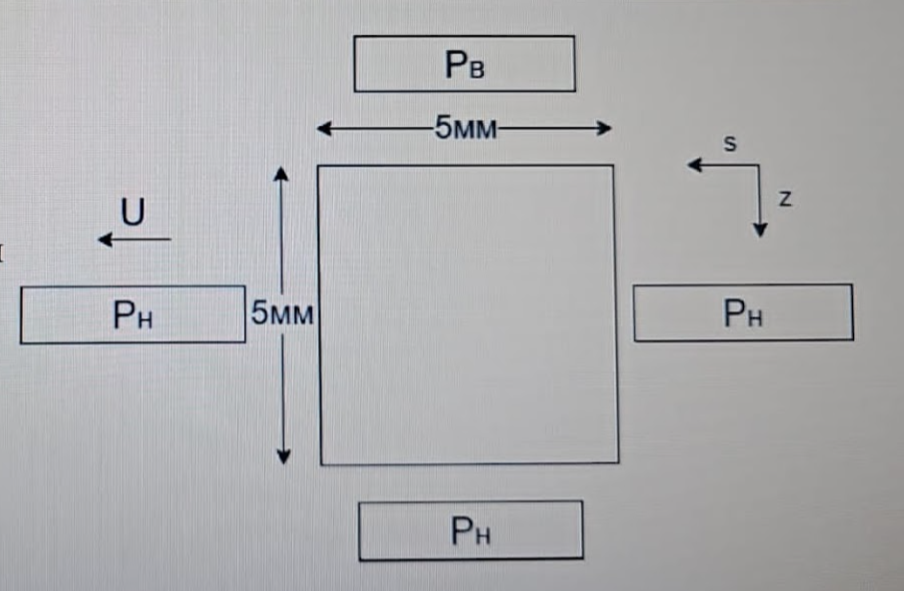
\includegraphics[width=\textwidth, height=0.5\textwidth]{taskGU.png}}
	\caption{Схема области решения и граничных условий уравнения Рейнольдса}
	\label{obl_resh}
\end{figure}

\section{Вывод уравнения Рейнольдса}

Гидродинамические уравнения несжимаемой жидкости с
внутренним трением могут быть представлены в очень простой
форме, если пренебречь силами, пропорциональными массам,
равно как и силами инерции.

Обозначая через $x$, $y$, $z$ прямоугольные координаты точки, через $p$ -- гидродинамическое давление в этой точке,

Силы трения $p_{xy}, p_{xz}, p_{yx}, p_{yz}, p_{zx}, p_{zy}$, перпендикулярные к оси силы, обозначенной первой буквой индекса и параллельные оси силы, обозначенной второй буквой индекса.

Обозначим проекции скорости на осях $x, y, z \text{ соответственно}$ $u, \nu, \omega$.

Введем $\mu$ как коэффициент внутреннего трения жидкости.ы
 Тогда можно записать три системы уравнений:
\begin{enumerate}
	\item Система, определяющая гидродинамическое давление в
	точке $x, y, z$:
	\begin{equation}
		\label{eqfi}
		\begin{cases}
			\frac{\partial p}{\partial x} = \mu \left( \frac{\partial^2 u}{\partial x^2} + \frac{\partial^2 u}{\partial y^2} + \frac{\partial^2 u}{\partial z^2} \right), \\
				\frac{\partial p}{\partial y} = \mu \left( \frac{\partial^2 \nu}{\partial x^2} + \frac{\partial^2 \nu}{\partial y^2} + \frac{\partial^2 \nu}{\partial z^2} \right), \\
					\frac{\partial p}{\partial z} = \mu \left( \frac{\partial^2 \omega}{\partial x^2} + \frac{\partial^2 \omega}{\partial y^2} + \frac{\partial^2 \omega}{\partial z^2} \right).
		\end{cases}
	\end{equation}
\item Система, определяющая силы трения в той же точке:
\begin{equation}
	\label{eqsi}
	\begin{cases}
		p_{yz} = p_{zy} = \mu \left(\frac{\partial \omega}{\partial y} + \frac{\partial \nu}{\partial z} \right), \\
			p_{zx} = p_{xz} = \mu \left( \frac{\partial \omega}{\partial x} +  \frac{\partial u}{\partial z} \right), \\
				p_{xy} = p_{yx} = \mu \left(  \frac{\partial u}{\partial y} + \frac{\partial \nu}{\partial x} \right).
	\end{cases}
\end{equation}
\item Условие несжимаемости жидкости, выраженное уравнением: 
\begin{equation}
	\label{eqthi}
	\frac{\partial u}{\partial x} + \frac{\partial \nu}{\partial y} + \frac{\partial \omega}{\partial z} = 0.
	\end{equation}

\end{enumerate}

Примем, что скорость $\nu = 0$, поскольку она мала по сравнению со скоростями $u = 0$, $\omega = 0$.

Изменения скоростей $u$ и $\omega$ со при заданном значении $y$ для всех изменений $ x $ и $z$ могут рассматриваться как чрезмерно малые, поэтому примем
\[
\frac{\partial^2 u}{\partial x^2} = 0, 
\frac{\partial^2 u}{\partial z^2} = 0, 
\frac{\partial^2 \omega}{\partial x^2} = 0, 
\frac{\partial^2 \omega}{\partial z^2} = 0. 
\]

Ограничиваясь приближенным решением, которое можно
получить при указанных выше предположениях, уравнения \eqref{eqfi}, \eqref{eqsi} и \eqref{eqthi} могут быть приведены к следующей форме.
\begin{equation}
	\label{secondinitialeq}
	\begin{cases}
		\frac{\partial p }{\partial x} = \mu \frac{\partial^2 u}{\partial y^2}, \\
		\frac{\partial p }{\partial y} = 0, \\
		\frac{\partial p }{\partial z} = \mu \frac{\partial^2 \omega}{\partial y^2}.
	\end{cases}
\end{equation}
\begin{equation}
	\label{secinitialeq}
	\begin{cases}
		p_{yz} = p_{xy} = \mu \frac{\partial \omega}{\partial y}, \\
		p_{zx} = p_{xz} = 0, \\
		p_{xy} = p_{yx} = \mu \frac{\partial u}{\partial y}.
	\end{cases}
\end{equation}
\begin{equation*}
	\frac{\partial u}{\partial x} + \frac{\partial \nu}{\partial y} + \frac{\partial \omega}{\partial z} = 0.
\end{equation*}

Для определения давления необходимо интегрировать выражения \eqref{secondinitialeq}, \eqref{secinitialeq}. Для этого определим граничные условия.

\noindent Для $y = 0$ имеем
\[
\begin{cases}
u = U_0, \\
 \nu = 0, \\
  \omega = 0.
\end{cases}
\]

\noindent Для $y = h$ имеем
\[
\begin{cases}
u = U_1, \\ 
\nu = U_1 - U_1 \frac{\partial  h}{\partial h}, \\ \omega = 0.
\end{cases}
\]

Поскольку $p$ не зависит от $y$, то интегрирование уравнений \eqref{secondinitialeq} приводит к уравнениям
\begin{equation}
	\label{1-inte-inti}
	\begin{cases}
		u = \frac{1}{2 \mu} \frac{\partial p}{\partial x} \left( y - h \right) y + U_0 \frac{h - y}{h} + U_1 \frac{y}{h},\\
		\omega = \frac{1}{2 \mu} \frac{\partial p}{\partial z} (y - h) y.
	\end{cases}
\end{equation} 
Первые производные вторых членов этих уравнений, перенесенные в соответствующие уравнения группы \eqref{secinitialeq}, приводят
к уравнениям
\begin{equation}
	\label{sec-init-eq}
	\begin{cases}
		p_{yz} = p_{zy} = \frac{1}{2} \frac{\partial p}{\partial z} \left( 2y - h \right), \\
		p_{xy} = p_{yz} = \frac{1}{2} \frac{\partial p}{\partial x} \left( 2y - h \right) + \mu \frac{U_1 - U_0}{h}.
	\end{cases}
\end{equation}

Если давление $p$ считать независимым от координаты $z$, то четыре последних
уравнения сокращаются до двух: первое из системы~\eqref{1-inte-inti} и
второе из системы~\eqref{sec-init-eq}.

Взяв производные от первого из этих уравнений по $x$ и
от второго по $z$ и подставляя это в уравнение~\eqref{eqthi}, находим, что
\begin{equation*}
		\frac{\partial \nu}{\partial y} = - \frac{1}{2 \mu} \left( \frac{\partial}{\partial x} \left( \frac{\partial p}{\partial x} (y - x) y \right) + \frac{\partial}{\partial z} \left( \frac{\partial p}{\partial z} (y - h) h \right) - \frac{\partial}{\partial x} \left( U_0 \frac{h - y}{h} + U_1 \frac{y}{h} \right) \right).
\end{equation*}

Интегрируя это уравнение в пределах от $y = 0$ до $y = h$ и
принимая во внимание граничные условия, получаем
\begin{equation*}
	\frac{\partial}{\partial x} \left( h^3 \frac{\partial p}{\partial x} \right) + \frac{\partial}{\partial z} \left( h^3 \frac{\partial p}{\partial z} \right) = 6 \mu \left( (U_0 - U_1) \frac{\partial h}{\partial x} \right) + 2 V_1.
\end{equation*}
$2 V_1$ используется для учёта движений одной из стенок зазора, меняющих значение функции. Если пренебречь этим, и обозначить $U_0 - U_1$ как $U$, то получим искомое уравнение~\eqref{reinolts-task}.

\section{Метод конечных элементов}

Основная идея метода конечных элементов состоит в том, что любую непрерывную величину, такую как температура, давление и перемещение, можно аппроксимировать дискретной моделью, которая строится на множестве кусочно-непрерывных функций, определенных на конечном числе подобластей. Кусочно-непрерывные функции определяются с помощью значений непрерывной величины в конечном числе точек рассматриваемой области.
В общем случае непрерывная величина заранее неизвестна и нужно определить значения этой величины в некоторых внутренних точках области. Дискретную модель, однако, не сложно построить, если сначала предположить, что числовые значения этой величины в каждой внутренней точке области известны. После этого можно перейти к общему случаю. Итак, при построении дискретной модели непрерывной величины поступают следующим образом:
\begin{enumerate}
	\item В рассматриваемой области фиксируется конечное число точек. Эти точки называются узловыми точками или просто узлами.
	\item Значение непрерывной величины в каждой узловой точке считается переменной, которая должна быть определена.
	\item Область определения непрерывной величины разбивается на конечное число подобластей, называемых элементами. Эти элементы имеют общие узловые точки и в совокупности аппроксимируют форму области.
	\item Выбор функций формы и аппрокисмирующей функции.
	\item Построение локальной матрицы.
	\item Построение глобальной матрицы путем сшивания локальных матриц элементов друг с другом.
	\item Учет граничных условий путем заменой коэффициентов в полученной матрице или же вектора правых частей.
	\item Решение системы линейных уравнений для получения решения в узловых точках.
\end{enumerate}

\subsection{Методика решения уравнения Рейнольдса с помощью слабой формы Галеркина}

Существуют разные подходы к реализации идеи метода конечных элементов. В данной работе рассмотрим методику решения с помощью слабой формы Галеркина. Для разбиения области на элементы требуется выбрать форму элемента. Поскольку рассматриваемая область прямоугольная, то удобно взять элементы прямоугольной формы. Пусть $l$ --- горизонтальная длинная области, а $h$ --- вертикальная. Тогда функции формы будут иметь следующий вид:
\begin{equation}
	\begin{cases}
		N_1 = 1 - \frac{x}{l} - \frac{z}{h} + \frac{x  z}{l  h}, \\
		N_2 = \frac{x}{l} - \frac{x  z}{l  h}, \\
		N_3 = \frac{x  z}{l h}, \\
		N_4 = \frac{z}{h} - \frac{x  z}{l  h}. \\
	\end{cases}
\label{form-func}
\end{equation}

Аппроксимирующую функцию зададим в виде:
\begin{equation*}
	\phi = c_0 N_1 + c_1 N_2 + c_2 N_3 + c_3 N_4.
\end{equation*}

Далее будем искать локальную матрицу из выражения:
\begin{equation*}
	\int_{S_i} {[N] \left(\frac{\partial}{\partial x} \left(h^3 \frac{\partial p}{\partial x} \right) + \frac{\partial}{\partial z} \left(h^3 \frac{\partial p}{\partial z} \right) - 6 \mu U \frac{\partial h}{\partial x}\right) dx dz} = 0.
\end{equation*}
$S_i$ --- область, содержащая элемент. 
Подставим аппрокисимирующую функцию $\phi$ вместо $p$.
\begin{equation*}
	\int_{S_i} {[N] \left(\frac{\partial}{\partial x} \left(h^3 \frac{\partial \phi}{\partial x} \right) + \frac{\partial}{\partial z} \left(h^3 \frac{\partial \phi}{\partial z} \right) - 6 \mu U \frac{\partial h}{\partial x}\right) dx dz} = 0.
\end{equation*}
Далее рассмотрим сумму интегралов:
\begin{equation*}
	\int_{S_i} {[N] \left(\frac{\partial}{\partial x} \left(h^3 \frac{\partial \phi}{\partial x} \right)\right) dx dz}
	+
	\int_{S_i} {[N] \left(\frac{\partial}{\partial z} \left(h^3 \frac{\partial \phi}{\partial z} \right)\right) dx dz} 
	-
	\int_{S_i} [N]\left(6 \mu U \frac{\partial h}{\partial x}\right) dx dz = 0.
\end{equation*}
Будем вычислять интегралы в которых участвует функция $\phi$ по частям:
\begin{equation*}
	\int_{S_i} {[N] \left(\frac{\partial}{\partial x} \left(h^3 \frac{\partial \phi}{\partial x} \right)\right) dx dz} = [N] h^3 \frac{d \phi}{dx}\Biggr|_{S_i} - \int_{S_i} {\frac{d[N]}{dx} \left(h^3 \frac{\partial \phi}{\partial x} \right) dx dz},
\end{equation*}
\begin{equation*}
	\int_{S_i} {[N] \left(\frac{\partial}{\partial z} \left(h^3 \frac{\partial \phi}{\partial z} \right)\right) dx dz} = [N] h^3 \frac{d \phi}{dz}\Biggr|_{S_i} - \int_{S_i} {\frac{d[N]}{dz} \left(h^3 \frac{\partial \phi}{\partial z} \right) dx dz}.
\end{equation*}
Суть такого подхода в том, что мы снижаем требования по дифференцируемости со второго до первого порядка.

После вычислений этих интегралов и их сложении можно получить матричное уравнение в локальных координатах относительно $\phi$ следующего вида:
\begin{equation}
W_i \phi = F_i,
\label{ref_local}
\end{equation}
где $F_i$ - правая часть, полученная из интеграла, не содержащего $\phi$:
\begin{equation*}
	F_i = \int_{S_i} [N]\left(6 \mu U \frac{\partial h}{\partial x}\right) dx dz.
\end{equation*}

Для вычисления глобальной матрицы требуется для каждого элемента подставить в вырождение~(\ref{ref_local}) для локальных координат узловые границы области и вычислить их значения. 
Далее нужно объединить все матрицы полученные в одну глобальную.

После объединения получаем матричное уравнение 
\begin{equation*}
	W \phi = F,
\end{equation*}

Далее заменяем значения в матрице $F$ и матрице $W$ так, чтобы решения совпадали с граничными условиями.
После подстановки граничных условий решением уравнения будут являться искомые значения давления $p$ в узловых точках.

\section{Программная реализация решения уравнения Рейнольдса методом конечных элементов}

Рассмотрим задачу со следующими входными данными 
\begin{equation*}
	\begin{cases}
		h = 0.0001 \text{ м}, \\
		verticalLength = 0.005 \text{ м}, \\
		horizontalLength = 0.005 \text{ м}, \\
		\mu = 8.90 * 10^{-4} \text{ Па}*\text{с}, \\
		U = 10 \text{ м/c}, \\
		p_{\text{н}} = 100 \text{ кПа}, \\
		p_{\text{в}} = 150 \text{ кПа}, \\
	\end{cases}	
\end{equation*}
$\mu$ --- коэффициент вязкости воды.

\subsection{Сетка 10 на 10 элементов}

Для сетки 10 на 10 элементов получаем следующие значения графики:

\begin{figure}[!htbp]
	\center{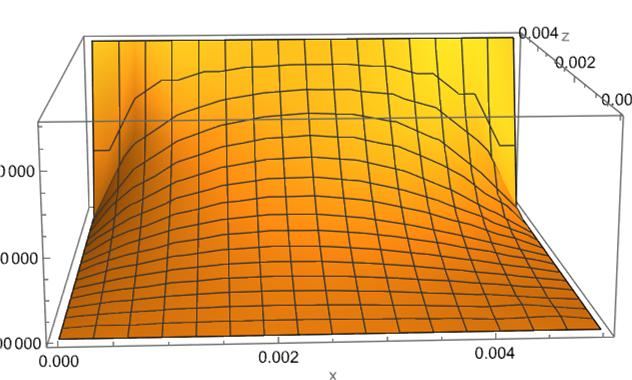
\includegraphics[width=\textwidth, height=0.5\textwidth]{10x10mesh.jpg}}
	\caption{График решения уравнения Рейнольдса для h = 0.0001 м на сетке 10 на 10 элементов}
	\label{10x10mesh}
\end{figure}
\begin{figure}[!htbp]
	\center{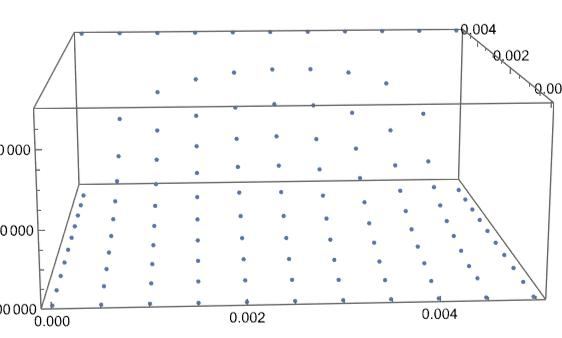
\includegraphics[width=\textwidth, height=0.5\textwidth]{10x10points.jpg}}
		\caption{График значений узлов решения уравнения Рейнольдса для h = 0.0001 м на сетке 10 на 10 элементов}
	\label{10x10points}
\end{figure}

Из полученных графиков видно, что граничные условия выполняются.

\newpage

\subsection{Сетка 20 на 20 элементов}

Для сетки 20 на 20 элементов получаем следующий   график решения

\begin{figure}[!htbp]
	\center{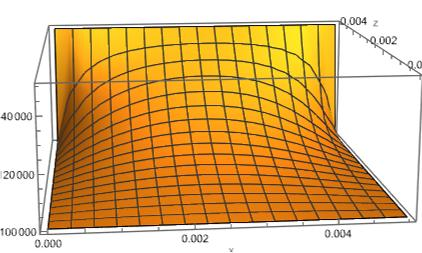
\includegraphics[width=\textwidth, height=0.5\textwidth]{20x20mesh.jpg}}
	\caption{График решения уравнения Рейнольдса для h = 0.0001 м на сетке 20 на 20 элементов}
	\label{20x20mesh}
\end{figure}
\begin{figure}[!htbp]
	\center{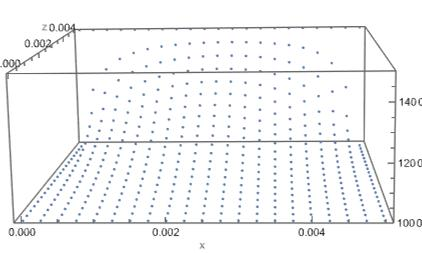
\includegraphics[width=\textwidth, height=0.5\textwidth]{20x20points.jpg}}
	\caption{График значений узлов решения уравнения Рейнольдса для h = 0.0001 м на сетке 20 на 20 элементов}
	\label{20x20points}
\end{figure}

Из полученных значений и графиков видно, что граничные условия выполняются.

\subsection{Сравнение полученного решения с решением Wolfram Mathematica}

Проверим полученный результат с помощью функции NDSolve в Wolfram Mathematica.

\begin{figure}[!htbp]
	\center{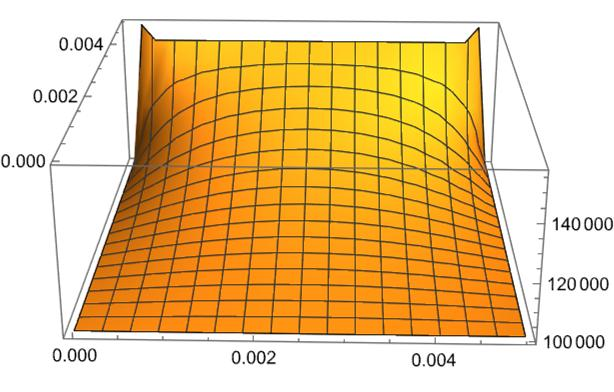
\includegraphics[width=\textwidth, height=0.5\textwidth]{exactSolutionConst.jpg}}
	\caption{График решения уравнения Рейнольдса для h = 0.0001 м полученный с помощью Wolfram Mathematica}
	\label{exactSolutionConst}
\end{figure}

Сравним решения полученные с помощью собственной реализацией с решением Wolfram Mathematica.

\begin{table}[!htbp]
	\begin{tabular}{|l|l|l|}
		\hline
		\multicolumn{1}{|c|}{Размерность сетки} & \multicolumn{1}{c|}{Разность, Па} & Погрешность, \% \\ \hline
		5 на 5                                  & 4612                              & 4.51            \\ \hline
		10 на 10                                & 1538                              & 1.38            \\ \hline
		20 на 20                                & 1290                              & 1.02            \\ \hline
	\end{tabular}
\end{table}

Погрешность была вычислена по формуле $\underset{i}{\max} | \frac{{x_w}_i - {x_{node}}_i}{{x_w}_i} |$, где ${x_w}_i$ -- значение в узле $i$, полученное в Wolfram Mathematica, а ${x_{node}}_i$ -- значение в узле $i$, полученное в созданной программе. Максимум вычисляется по всем узловым элементам.

Можно заметить, что полученное решение отличается не более чем на 4.51 \%, с увеличением числа элементов в сетке погрешность падает. Это свидетельствует о верности полученного решения. 

\newpage
\section-{Заключение}
В работе представлен вывод уравнения Рейнольдса для установившегося течения в газовом смазочном слое и методика решения уравнения Рейнольдса с помощью метода конечных элементов. В ходе работы получены следующие результаты:
	\begin{enumerate}	
		\item Создана программная реализация метода конечного элемента для решение уравнения Рейнольдса
		\item Полученные значения решения уравнения Рейнольдса были сравнены с результатами решения, полученного с помощью функции NDSolve в Wolfram Mathematica
		\item В результате сравнения для сетки 5 на 5 погрешность равна 4.51 \%, а для сетки 20 на 20 -- 1.02 \%.
	\end{enumerate}

\newpage
\begin{thebibliography}{2}
\bibitem{petrov_smazka} Петров Н. Гидродинамическая теория смазки, М.: из-во академии наук СССР, 1948. --- 558~с.
\bibitem{slezkin_smazka} Слезкин Н. Динамика вязкой несжимаемой жидкости, М.: из-во техно-теоретической литературы, 1955. --- 521~с.
\bibitem{seligard} Селегринд Л. Примененение метода конечных элементов, М.: из-во МИР, 1979. --- 195~с.
\bibitem{seshu} Seshu P. Textbook of
Finite Element
Analysis, М.: PHI Learning Private Limited, 2012. --- 340~с.

\end{thebibliography}

\end{document} 